\documentclass{article}
\usepackage{amsfonts, amsmath, amssymb, amsthm} % Math notations imported
\usepackage{enumitem}
\usepackage[margin=1in]{geometry}
\usepackage{graphicx}
\usepackage{subfig}
\graphicspath{{./images/}} % Path to images

\newtheorem{thm}{Theorem}
\newtheorem{prop}[thm]{Proposition}
\newtheorem{cor}[thm]{Corollary}

% title information
\title{Math 154 HW4}
\author{Neo Lee}
\date{05/03/2023}

% main content
\begin{document} 

% placing title information; comment out if using fancyhdr
\maketitle 
\textbf{Problem 1.}
\begin{figure}[htb]
    \qquad
    \begin{minipage}{.4\textwidth}
        \centering
        {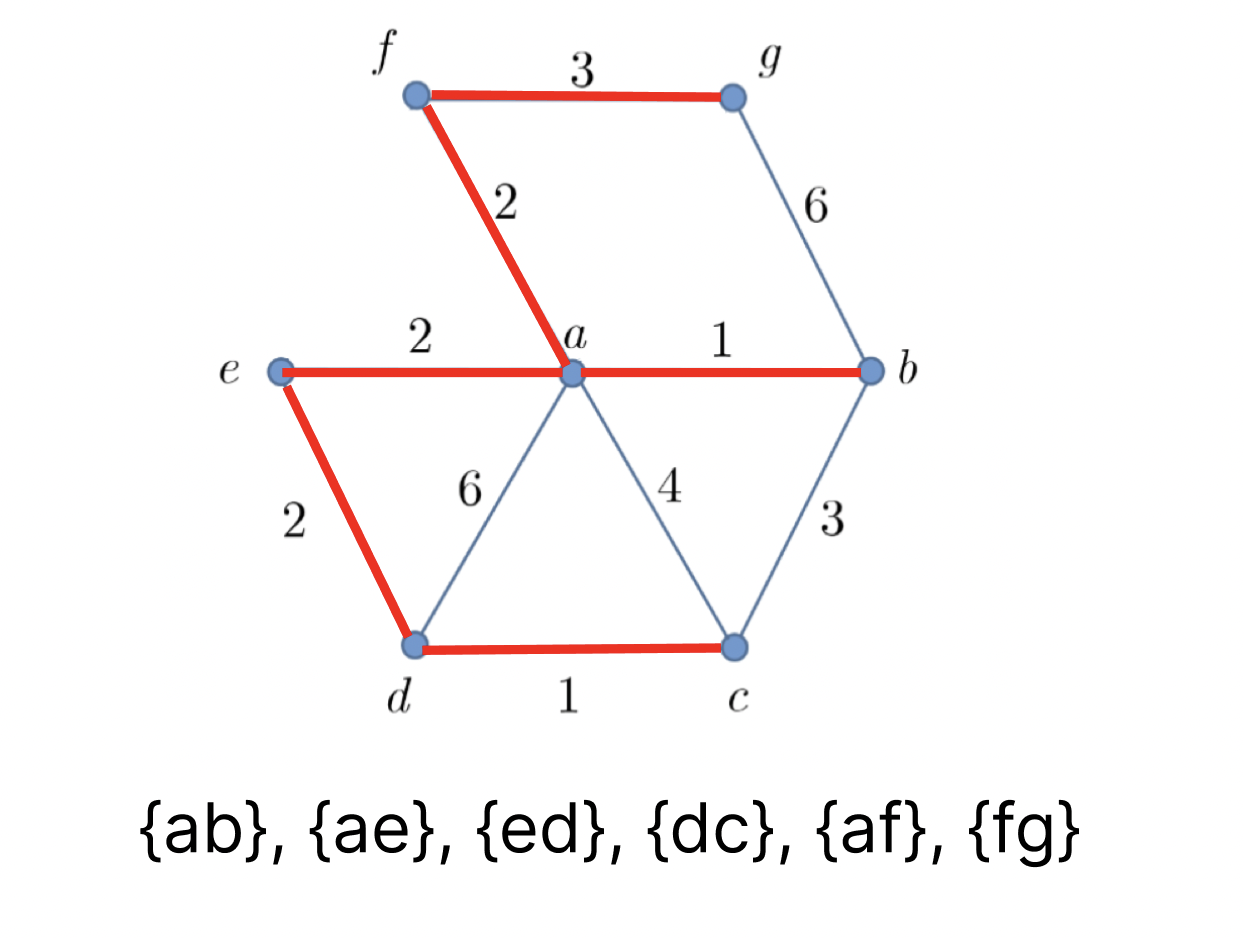
\includegraphics[scale=0.35]{prims.png}}
        \qquad\qquad\emph{Prim's}\label{fig:1}
    \end{minipage}    
    \qquad
    \begin{minipage}{.4\textwidth}
        \centering
        {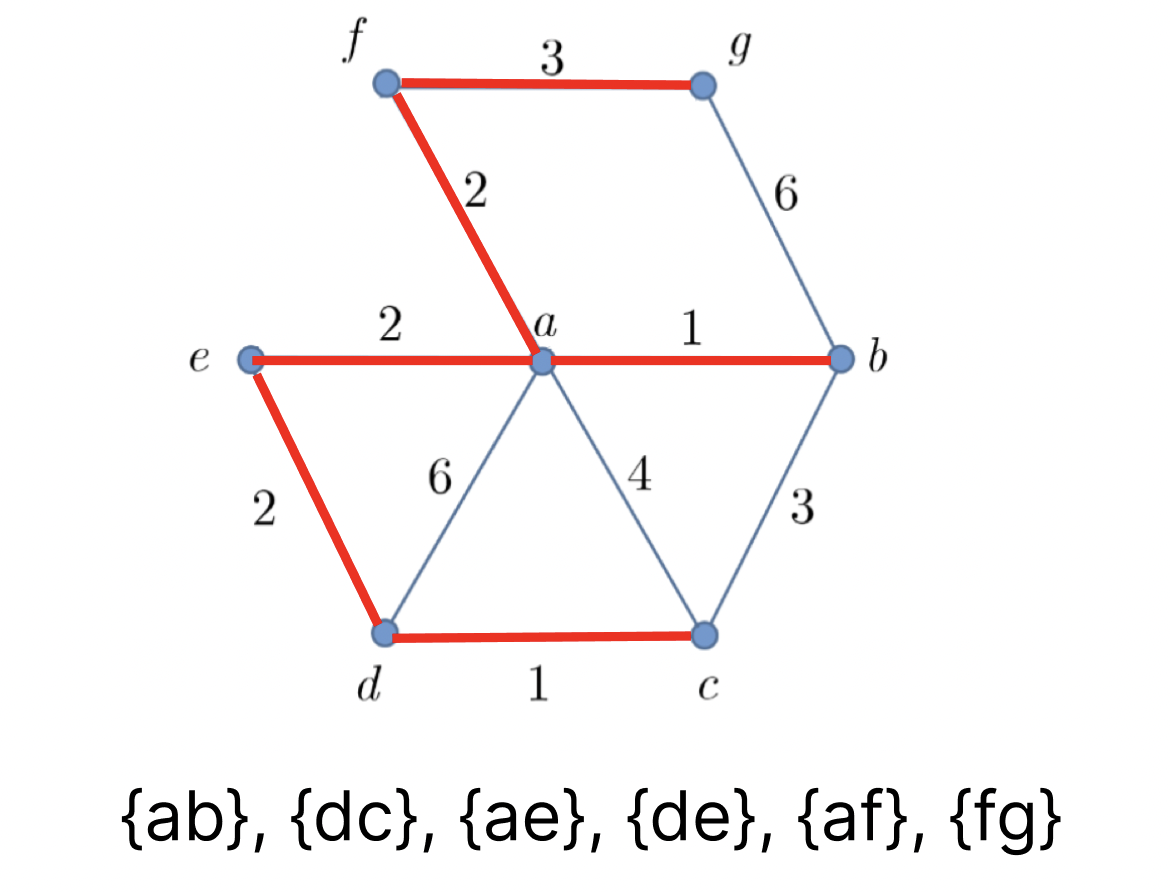
\includegraphics[scale=0.35]{kruskal.png}}
        \qquad\qquad\emph{Kruskal's}\label{fig:2}
    \end{minipage}        
\end{figure} 
\bigbreak

\textbf{Problem 2.}
\begin{enumerate}[label=(\alph*)]
    \item Let $v_1, v_2, v_3, v_4$ be the only vertices in the graph $G$ with edges $\{v_1, v_2\}$ and $\{v_3, v_4\}$ only.
    Then all vertices have degree one but the graph is disconnected.

    \item
    The proof using induction inherently assumed that all graphs are constructed algorithmically by adding one vertex each at a time. 
    However, it overlooked the case where the graph can be constructed by adding multiple vertices at a time, and the condition of having at least degree one will still be true.
    Hence, the proof is not exhaustive.
\end{enumerate}
\bigbreak

\textbf{Problem 3.}

\begin{prop}
    $Q_n$ is bipartite for all $n \geq 2$.
\end{prop}
\begin{proof}
    We will prove by induction.

    \underline{Base case:} $n = 2$. $n=2$ only have 4 vertices in total and can be checked to be true easily.

    \underline{Inductive step:} Assume $Q_n$ is bipartite. We will show that $Q_{n+1}$ is bipartite as well.
    Notice that all $Q_{n+1}$ can be constructed by making a copy of $Q_n$, let $Q'_n$, and connecting the corresponding vertices in $Q_n$ and $Q'_n$.

    To illustrate more clearly with examples, let all vertices of $Q_n$ be $0x_1x_2\dots x_n$ and those of $Q'_n$ be $1x_1x_2\dots x_n$ with $x_i$ taking values 0 or 1.
    By inductive hypothesis, we know both $Q_n$ and $Q'_n$ are bipartite. Then, we just need to connect the corresponding vertices in $Q_n$ and $Q'_n$ to form $Q_{n+1}$.

    Since $Q'_n$ is a copy of $Q_n$, they have the same labeling of vertices. 
    Then, we just need to flip the labeling of $Q'_n$ and connect it to $Q_n$ by adding the new edges. 
    Since the vertices of $Q_n$ and $Q'_n$ are one-bit different, e.g. $010101$ to $110101$, the only new edges are the ones between the one-to-one corresponding vertices.
    Because we have flipped the labeling of $Q'_n$, the new edges are between vertices of different labels, and the entire $Q_{n+1}$ are labeled with alternating labels.

    Hence, $Q_{n+1}$ is bipartite.

    \underline{By Mathematical Induction}, $Q_n$ is bipartite for all $n \geq 2$.
\end{proof}
\bigbreak

\begin{prop}
    $Q_n$ contains at least $2\cdot \left(2^{2^{n-1}}\right)-1$ independent sets, for all $n\ge 2$.
\end{prop}
\begin{proof}
    Proof goals: $Q_n$ is bipartite $\Rightarrow$ parts $A, B$ have same number of vertices $\Rightarrow$ parts $A, B$ are independent sets $\Rightarrow$ subsets of $A, B$ are also independent sets.

    From \emph{Proposition 1}, we have already proved that $Q_n$ is bipartite. 
    Then from the inductive step in \emph{Prop 1}, we have flipped the labeling of the copy graph, so the new Hypercube Graph has $|A'| = |A| + |B| = |B'|$. 
    Indeed, the parts $A', B'$ have the same number of vertices, which is true for all $Q_n$.

    Then, by definition of bipartite graph, all vertices exclusively in $A$ or $B$ are disjoint, which means $A, B$ are themselves independent sets. 
    Then, obviously all subsets of independent sets $A, B$ are also independent sets.

    Now, let's just count the number of independent sets in $A$. 
    $A$ has half the number of total vertices, $2^{n-1}$, and the power set of $A$ has $2^{2^{n-1}}$ elements.
    Now we do the same for $B$, so in total there are $2\cdot \left(2^{2^{n-1}}\right)$ sets, since we double counted empty set, so it's just $2\cdot \left(2^{2^{n-1}}\right)-1$ in total. 
    These are the sets that are guaranteed to be independent sets. Hence, we proved the weak inequality.
\end{proof}
\bigbreak

\textbf{Problem 4.}
\begin{prop}
    A tree has at most one perfect matching.
\end{prop}
\begin{proof}
    Suppose that a tree $T$ has at least two perfect matchings $M$ and $M'$. 
    Since a leaf $u$ only has one edge, it must be matched to it's parent $v$, and so $\{u, v\} \in M, M'$.
    We can then remove $u, v$ from $T$, and the resulting graph is still a tree with perfect matching.
    We iterate the process above until we can not remove any more matchings. Since the resulting trees have even number of vertices 
    and have at least one leaf, we can always remove an edge containing a leaf that is in both $M$ and $M'$ until $T$ is empty, and so $M = M'$.
\end{proof}

\end{document}